%# -*- coding: utf-8 -*-
%!TEX encoding = UTF-8 Unicode
%!TEX TS-program = xelatex
% vim:ts=4:sw=4
%
% 以上设定默认使用 XeLaTex 编译,并指定 Unicode 编码,供 TeXShop 自动识别

%第二回 
\chapter{西門慶簾下遇金蓮\KG 王婆貪賄說風情}

「月老姻緣配未真,  金蓮賣俏逞花容,

只因月下星前意,  惹起門旁簾外心;

王媽誘財施巧計,  鄆哥賣果被嫌嗔,

那知後日蕭墻禍,  血濺屏幃滿地紅。」

話說武松自從搬離哥後,撚指不覺雪晴,過了十數日光景。都說本縣知縣,自從到任以來,都得二年有餘,
轉得許多金銀,
\jiaoMJ{(轉得許多金銀)「轉」容本《忠義水滸傳》做「撰」,稍後如楊定見本、芥子園本、金聖歎貫華堂七十回本水滸傳均做「賺」。而前此世德堂本《西遊記》,已用「賺」代「撰」。本書「轉」、「撰」、「賺」並用。第五十三回:「賺得些中錢,又來撒漫了」;第七十六回:「家中胡亂積賺了些小本經紀」;第九十八回:「別無生意,只靠老婆錢賺」。下凡「轉」、「撰」取錢物,均統一為「賺」,不再一一出校。}
要使一心腹人,送上東京親眷處收寄。三年任滿朝覲,打點上司。一來都怕路上小人,須得一個有力量的人去方好。猛可想起都頭武松,須得此人英雄膽力,方了得此事。當日就喚武松到衙內商議,道:「我有個親戚,在東京城內做官,姓朱名勔,見做殿前太尉之職。要送一擔禮物,
稍封書
\jiaoMJ{(稍封書)「稍」此處代「捎」。劉改「捎」。下凡以「稍」代「捎」,隨文改正,不再出校。}
去問安。只恐途中不好行,須得你去方可。你休推辭辛苦,回來我自重賞你!」武松應道:「小人得蒙恩相抬舉,安敢推辭?既蒙差遣,只得便去。小人自來也不曾到東京,就那裡觀光上國景致,走一遭,也是恩相抬舉。」知縣大喜,賞了武松三盃酒,十兩路費,不在話下。

且說武松領了知縣的言語,出的縣門來,到下處叫了士兵,都來街上買了一瓶酒,并菜蔬之類,逕到武大家。武大恰街上回來,見武松在門前坐地,交士兵去廚下安排。那婦人餘情不斷,見武松把將酒食來,心中自思:「莫不這廝思想我了,不然都又回來?那廝一定強我不過,我且慢慢問他。」婦人便上樓去,重勻粉面,再挽雲鬟,換了些顏色衣服穿了,來到門前迎接武松。婦人拜道:「叔叔不知怎的錯見了,好幾日並不門,交奴心裡沒理會處!每日交你哥哥去縣裡尋叔叔陪話,歸來只說沒尋處。今日再喜得叔叔來家,沒事壞鈔做甚麼?」武松道:「武二有句話,特來要和哥哥說知。」婦人道:「既如此,請樓上坐。」

三個人來到樓上,武松讓哥嫂上首坐了,他便掇杌子打橫。士兵擺上酒來,熱下飯。一齊拏上來。武松勸哥嫂吃,婦人便把眼來睃武松,武松只顧吃酒。酒至數巡,武松問迎兒討副勸盃,叫士兵篩一盃酒,拏在手裡,看著武大道:「大哥在上,武二今日蒙知縣相公差往東京幹事,明日便要起程。多是兩三個月,少是一個月便回。有句話特來和你說,你從來為人懦弱,我不在家,恐怕外人來欺負。假如你每日賣十扇籠炊餅,你從明日為始,只做五扇籠炊餅出去賣。每日遲出早歸,不要和人吃酒。歸家便下了簾子,早閉門,省了多少是非口舌。若是有人欺負你,不要和他爭執,待我回來,自和他理論。大哥你依我時,滿飲此盃。」武大接了酒,道:「我兄弟見得是,我都依你說!」吃過一盃,武松再斟第二盞酒,對那婦人說道:「嫂嫂是個精細的人,不必要武松多說。我的哥哥,為人質朴,全靠嫂嫂做主。常言:『表壯不如裡壯』。嫂嫂把得家定,我哥哥煩惱做甚麼?豈不聞古人云:『籬牢犬不入』。」那婦人聽了這幾句話,一點紅從耳畔起。須臾,紫漒了面皮,指著武大罵道:「你這個混沌東西!有甚言語,在別人處說,來欺負老娘!我是個不戴頭巾的男子漢,叮叮噹噹響的婆娘,拳頭上也立得人,胳膊上走得馬,人面上行的人,不是那腲膿血,搠不出來鱉。老婆自從嫁了武大,真個螻蟻不敢入屋裡來。有甚麼籬笆不牢,犬兒鑽得入來!你休胡言亂語!一句句都要下落。丟下塊磚兒,一個個也要著地!」武松笑道:「若得嫂嫂這般做主,最好。只要心口相應,都不應心頭不似口頭。既然如此,我武松都記得嫂嫂說的話!請過此盃。」那婦人一手推開酒盞,一直跑下樓來,走到半胡梯上,發話道:「既是你聰明伶俐,恰不道長嫂為母!我初嫁武大時,不曾聽得有甚小叔,那裡走得來?是親不是親,便要做喬家公!

自是老娘悔氣了,偏撞著這許多鳥事!」一面哭下樓去了。有詩為證:

「苦口良言諫勸多,  金蓮懷恨起風波;

自家惶愧難存坐,  氣殺英雄小二哥!」

那婦人做出許多喬張致來。武大、武松吃了幾杯酒,坐不住,都下的樓來;弟兄洒淚而別。武大道:「兄弟去了,早早回來,和你相見。」武松道:「哥哥,你便不做買賣也罷,只在家裡坐的。盤纏兄弟自差人送與你。」臨行,武松又分付道:「哥哥,我的言語,休要忘了,在家仔細門戶!」武大道:「理會得了。」武松辭了武大,回到縣前下處,收拾行裝并防身器械。次日,領了知縣禮物、金銀、駝垜,討了腳程,起身上路,往東京去了。不題。只說武大自從兄弟武松說了去,整日乞那婆娘罵了三四日。武大忍氣吞聲,由他自罵,只依兄弟言語,每日只做一半炊餅出去。未晚便回家,歇了擔兒,先便去除簾子,關上大門,都來屋裡動彈。那婦人看了這般,心內焦燥起來,罵道:「不識時濁物!我倒不曾見日頭在半天裡,便把牢門關了,也吃鄰舍家話。說我家怎生禁鬼!聽信你兄弟說,空生有卵鳥嘴,也不怕別人笑恥!」武大道:「由他笑也罷,我兄弟說的是好話,省了多少是非。」被婦人噦在臉上道:「呸!濁東西!你是個男子漢,自不做主,都聽別人調遣!」武大搖手道:「由他,我兄弟說的金石之語!」原來武松去後,武大每日只是晏出早歸,到家便關門。那婦人氣生氣死,和他合了幾場氣,落後鬧慣了。自此婦人約莫武大歸來時分,先自去收簾子,關上大門,武大見了,心裡自也暗喜,尋思道:「恁的都不好!」有詩為證:

「慎事關門并早歸,  眼前恩愛隔崔嵬;

春心一點如絲亂,  空鎖牢籠總是虛。」

白駒過隙,日月攛梭,纔見梅開臘底,又早天氣回陽。一日,三月春光明媚時分,金蓮打扮光鮮,單等武大出門,就在門前簾下站立,約莫將及他歸來時分,便下了簾子,自去房內坐的。一日也是合當有事,都有一個人從簾子下走過來。自古沒巧不成話,姻緣合當湊著。婦人正手裡拏著叉竿放簾子,忽被一陣風將叉竿刮倒,婦人手擎不牢,不端不正,卻打在那人頭巾上。婦人便慌忙陪笑。把眼看那人,也有二十五、六年紀,生的十分博浪。頭上戴著纓子帽兒,金玲瓏簪兒,金井玉欄杆圈兒。長腰身,穿綠羅褶兒。腳下細結底陳橋鞋兒,清水布襪兒。腿上勒著兩扇玄色挑絲護膝兒,手裡搖著洒金川扇兒,越顯出張生般龐兒,潘安的貌兒,可意的人兒,風風流流,從簾子下丟與奴個眼色兒。這個人被叉杆打在頭上,便立住了腳。待要發作時,回過臉來看,都不想是個美貌妖嬈的婦人。但見他:

黑鬢鬢賽鴉翎的鬟兒,翠灣灣的新月的眉兒,清冷冷杏子眼兒,香噴噴櫻桃口兒,直隆隆瓊瑤鼻兒,粉濃濃紅豔腮兒,嬌滴滴銀盆臉兒,輕嬝嬝花朵身兒,玉纖纖葱枝手兒,一捻捻楊柳腰兒,軟濃濃白面臍肚兒,窄多多尖趫腳兒,肉奶奶胸兒,白生生腿兒,更有一件緊揪揪紅縐縐白鮮鮮黑裀裀,正不知是什麼東西。觀不盡這婦人容貌,且看他怎生打扮?但見:

%䯼{髟狄}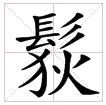
\includegraphics[width=20pt]{figure-char/diji.jpeg}
「頭上戴著黑油油頭髮䯼髻,口面上緝著皮金,一逕裡
【執足】
出香雲一結,周圍小簪兒齊插。六鬢斜插一朵並頭花,排草梳兒後押。難描八字灣灣柳葉,襯在腮兩朵桃花。玲瓏墜兒最堪誇,露賽玉酥胸無價;毛青布大袖衫兒,褶兒又短,襯湘裙碾絹綾紗。通花汗巾兒,袖中兒邊搭刺。香袋兒身邊低掛,抹胸兒重重紐扣,褲腿兒臟頭垂下。往下看,尖趫趫金蓮小腳,雲頭巧緝山牙。老鴉鞋兒白綾高底,步香塵偏襯登踏,紅紗膝褲扣鶯花。行坐處風吹裙袴,口兒裡常噴出異香蘭麝。櫻桃初笑臉生花,人見了魂飛魄散,賣弄殺偏俏的冤家」
%\piMINE{全书唯一的闪亮登场}

那人見了,先自酥了半邊,那怒氣早已鑽入爪哇國去了,變顏笑吟吟臉兒。這婦人情知不是,叉手望他深深拜了一拜,說道:「奴家一時被風失手,誤中官人,休怪。」那人一面把手整頭巾,一面把腰曲著地,還喏道:「不妨!娘子請方便。」卻被這間壁住的賣茶王婆子看見。那婆子笑道:「兀的誰家大官人,打這屋簷下過?打的正好!」那人笑道:「倒是我的不是,一時沖撞,娘子休怪。」婦人答道:「官人不要見責。」那人又笑著,大大的唱個喏,回應道:「小人不敢。」那一雙積年招花惹草,慣覷風情的賊眼,不離這婦人身上,臨去也回頭了七八遍,方一直搖搖擺擺,遮著扇兒去了。有詩為證:

「風日清和漫出遊,  偶從簾下識嬌羞;

只因臨去秋波轉,  若起春心不肯休。」

當時婦人見了那人生的風流浮浪,語言甜淨,更加幾分留戀。「倒不知此人姓甚名誰?何處居住?他若沒我情意時,臨去也不回頭七八遍了。不想這段姻緣,都在他身上!」都是在簾下,眼巴巴的看不見那人,方纔收了簾子,關上大門,歸房去了。看官聽說:莫不這人無有家業的?原是清河縣一個破落戶財主,就縣門前開著個生藥舖。從小兒也是個好浮浪子弟,使得些好拳棒,又會賭博,雙陸象棋,抹牌道字,無不通曉。近來發跡有錢,專在縣裏管些公事,與人把攬說事過錢,交通官吏,因此滿縣人都懼怕他。那人覆姓西門,單名一個慶字,排行第一,人都叫他做西門大郎。近來發跡有錢,人都稱他做西門大官人。他父母雙亡,兄弟俱無,先頭渾家是早逝,身邊止有一女。新近又娶了清河左衛吳千戶之女,填房為繼室,房中也有四五個丫鬟婦女。又常與抅攔裡的李嬌兒打熱。今也娶在家裡;南街子又占著窠子卓二姐,名卓丟兒,包了些時,也娶來家居住。專一飄風戲月,調占良人婦女,娶到家中,稍不中意,就令媒人賣了;一個月倒在媒人家去二十餘遍,人多不敢惹他。這西門大官人自從簾下見了那婦人一面,到家尋思道:「好一個雌兒!怎能勾得手?」猛然想起那間壁賣茶王婆子來,堪可如此如此,這般這般,撮合得此事成,我破幾兩銀子謝他,也不值甚的!于是連飯也不吃,走出街上閑遊,一直逕踅入王婆茶坊裡來,便去裡邊水簾下坐了。王婆笑道:「大官,都纔唱得好個大肥喏!」西門慶道:「乾娘,你且來,我問你。間壁這個雌兒是誰的娘子?」王婆道:「他是閻羅大王的妹子,五道將軍的女兒。問他怎的?」西門慶說:「我和你說正話,休取笑。」王婆道:「大官人怎的不認的?他老公便是縣前賣熟食的。」西門慶道:「莫不是賣棗糕徐三的老婆?」王婆搖手道:「不是。若是他,也是一對兒!大官人再猜。」西門慶道:「敢是賣餶飿的李三娘子兒?」王婆搖手道:「不是。若是他,倒是一雙!」西門慶道:「豈不是花胳膊劉小二的婆兒?」王婆大笑道:「不是。若是他時,又是一對兒!大官人再猜。」西門慶道:「乾娘,我其實猜不著了。」王婆冷冷笑道:「不是,若是他時,好交大官人得知了罷。」笑一聲。「他的蓋老,便是街上賣炊餅的武大郎。」西門慶聽了,跌腳笑道:「莫不是人叫他『三寸丁、谷樹皮』的武大郎麼?」王婆道:「正是他!」西門慶聽了,叫起苦來,說道:「好一塊羊肉,怎生落在狗口裡!」王婆道:「便是這般故事。自古駿馬都駝痴漢走,美妻常伴拙夫眼。月下老偏這等配合!」西門慶道:「乾娘,我少你多少茶果錢?」王婆道:「不多,由他,歇些時都筭不妨。」西門慶又道:「你兒子王潮,跟誰出去了?」王婆道:「說不的,跟了一個淮上客人,至今不歸,又不知死活。」西門慶道:「都不交他跟我,那孩子倒乖覺伶俐!」王婆道:「若得大官人抬舉他時,十分之好。」西門慶道:「待他歸來,都再計較。」說畢大謝,起身去了。約莫未及兩個時辰,又踅將來王婆門首簾邊坐的,朝著武大門前半歇。王婆出來道:「大官人,吃個梅湯 。」西門慶道:「最好,多加些酸味兒。」王婆做了個梅湯,雙手遞與西門慶吃了,將盞子放下。西門慶道:「乾娘,你這梅湯做得好,有多少在屋裡?」王婆笑道:「老身做了一世媒,那討得不在屋裡?」西門慶笑:「我問你這梅湯,你都說做媒,差了多少!」王婆道:「老身只聽得大官人問這媒做得好,老身道說做媒。」西門慶道:「乾娘,你既是撮合山,也與我做頭媒。說道好親事,我自重重謝你!」王婆道:「看這大官人作戲!你宅上大娘子得知,老婆子這臉上,怎乞得那等刮子!」西門慶道:「我家大娘子最好性格,見今也有幾個身邊人在家,只是沒一個中得我意的!你有這般好的,與我主張一個,便來說也不妨。若是回頭人兒也好,只是要中得我意。」王婆道:「前日有一個到,只怕大官人不要。」西門慶道:「若是好時,與我說成了,我自重謝你!」王婆道:「生的十二分人才,只是年紀大些。」西門慶道:「自古半老佳人可共。便差一兩歲,也不打緊。真個多少年紀?王婆子道:「那娘子是丁亥生,屬豬的,交新年恰九十三歲了。」西門慶笑道:「你看這風婆子,只是扯著風臉取笑!」說畢,西門慶笑了起身去。看看天色晚了,王婆都纔點上燈來。正要關門,只見西門慶又踅將來,逕去簾子底下,拿凳子上坐了,朝著武大門前,只顧將眼睃望。王婆道:「大官人,吃個和合湯 。」西門慶道:「最好,乾娘放甜些。」王婆連忙取一鐘來,與西門慶吃了。坐到晚夕,起身道:「乾娘記了帳目,明日一發還錢。」王婆道:「由他伏惟安置,來日再請過論。」西門慶笑了去,到家甚是寢食不安,一片心只在婦人身上。當晚無話。次日清晨,王婆都纔開門,把眼看外時,只見西門慶又早在街前來回踅走。王婆道:「這刷子踅得緊,你看我著些甜糖,抹在這廝鼻子上,交他抵不著!那廝全討縣裡人便益,且交他來娘手裡納些販鈔,撰他幾貫風流錢使。」原來這開茶坊的王婆子,也不是守本分的。便是積年通殷勤,做媒婆,做賣婆,做牙婆。又會收小的,也會抱腰,又善放刁。還有一件不可說,䯼髻上著綠,陽臘灌腦袋。端的看不出這婆子的本事來!但見:

「開言欺陸賈,出口勝隨。只憑說六國唇鎗,全使話三齊舌劍。隻鸞孤鳳,霎時間交仗成雙;寡婦鰥男,一度話搬唆擺對。解使三里門內女,遮麼九皈殿中仙。玉皇殿上,侍香金童,把臂拖來;王母宮中;傳言玉女,攔腰抱住。略施奸計,使阿羅漢抱住比丘尼;纔用機關,交李天王摟定鬼子母。甜言說誘,男如封涉也生心,軟語調和,女似麻姑須亂性。藏頭露尾,攛掇淑女害相思;送暖偷寒,調弄嫦娥偷漢子。這婆子,端的慣調風月巧排,常在公門操鬬毆。」

這婆子正開門,在茶局子裡整理茶鍋。張見西門慶踅過幾遍,奔入茶局子水廉下,對著武大門首,不住把眼只望簾子裡瞧。王婆只推不看見,只顧在茶局子內搧火,不出來問茶。西門慶叫道:「乾娘,點兩盃茶來我吃。」王婆道:「大官人來了!連日少見,且請坐。」不多時,便濃濃點兩盞稠茶,放在桌子上。西門慶道:「乾娘,相陪我吃了茶。」王婆哈哈笑道:「我又不是你影射的,緣何陪著你吃茶?」西門慶也笑了一會,便問:「乾娘,間壁賣的是甚麼?」王婆道:「他家賣的拖煎河漏子 、乾巴子肉 、翻包著菜肉匾食、餃窩窩 蛤蜊麵 、熱盪溫和大辣酥 。」西門慶笑道:「你看這風婆子,只是風!」王婆笑道:「我不是風,他家自有親老公。」西門慶道:「我和你說正話。他家如法做得好炊餅,我要問他買四五十個,拏的家去。」王婆道:「若要買他燒餅,少間等他街上回來買,何消上門上戶?」西門慶道:「乾娘說的是。」吃了茶,坐了一會,起身去了。良久,王婆只在茶局裡。比時冷眼張見他,在門前{執足}過,東看一看,又轉西去,又復一復,一連走了七八遍。少頃,逕入茶房裡來。王婆道:「大官人僥倖,好幾日不見面了。」西門慶便笑將起來,去身邊摸出一兩一塊銀子,遞與王婆,說道:「乾娘,權且收了,做茶錢。」王婆笑道:「何消得許多?」西門慶道:「多者乾娘只顧收著。」婆子暗道:「來了。這刷子當敗,且把銀子收了,到明日與老娘做房錢!」便道:「老身看大官人有些湯,吃了寬蒸茶兒如何?」西門慶:「如何乾娘便猜得著?」婆子道:「有甚難猜處?自古入門休問榮枯事,觀看形容便得知。老身異樣蹺蹊古怪的事,不知猜勾多少。」西門慶道:「我有一件心上的事,乾娘若猜得著時,便輸與你五兩銀子。」王婆笑道:「老娘也不消三智五猜,只一智,便猜個中節。大官人,你將耳朵來。你這兩日腳步兒勤,趕趁得頻,已定是計掛著間壁那個人,我這猜如何?」西門慶笑將起來,道:「乾娘,端的智賽隨何,機強陸賈。不瞞乾娘說,不知怎的,吃他那日叉簾子時見了一面,恰似收了我三魂六魄的一般,日夜只是放他不下。到家茶飯懶吃,做事沒入腳處。不知你會弄手段麼?」王婆冷冷笑道:「老身不瞞大官人說,我家賣茶,叫做鬼打更,三年前十月初三日下大雪那一日,賣了不泡茶 ,直到如今不發市,只靠些雜趁養口。」西門慶道:「乾娘,如何叫做雜趁?」王婆笑道:「老身自從三十六歲沒了老公,丟下這個小廝,無得過日子。迎頭兒跟著人說媒,次後攬人家些衣服賣,又與人家抱腰收小的。閒常也會做牽頭,做馬伯六,也會針炙看病,也會做貝戎兒。」西門慶聽了,笑將起來:「我並不知乾娘有如此手段!端的與我說這件事,我便送十兩銀子,與你做棺材本。你好交這雌兒會我一面。」王婆便哈哈笑了。有詩為證:

虧殺賣茶王老母,  生死巫女會襄王。」

畢竟婆子有甚計策說來?要知後項事情,且聽下回分解:




